\chapter{aCoral结构}

\section{aCoral系统结构}
aCoral由内核(kernel)和外围模块(Peripheral)两大部分组成。
其中内核又包含中断管理系统、内存管理系统、线程管理系统和线程交互系统;
外围模块包括驱动管理、图形用户界面(GUI)、文件系统和网络模块(Net)。
如图2-1所示。

\begin{figure}[H]
	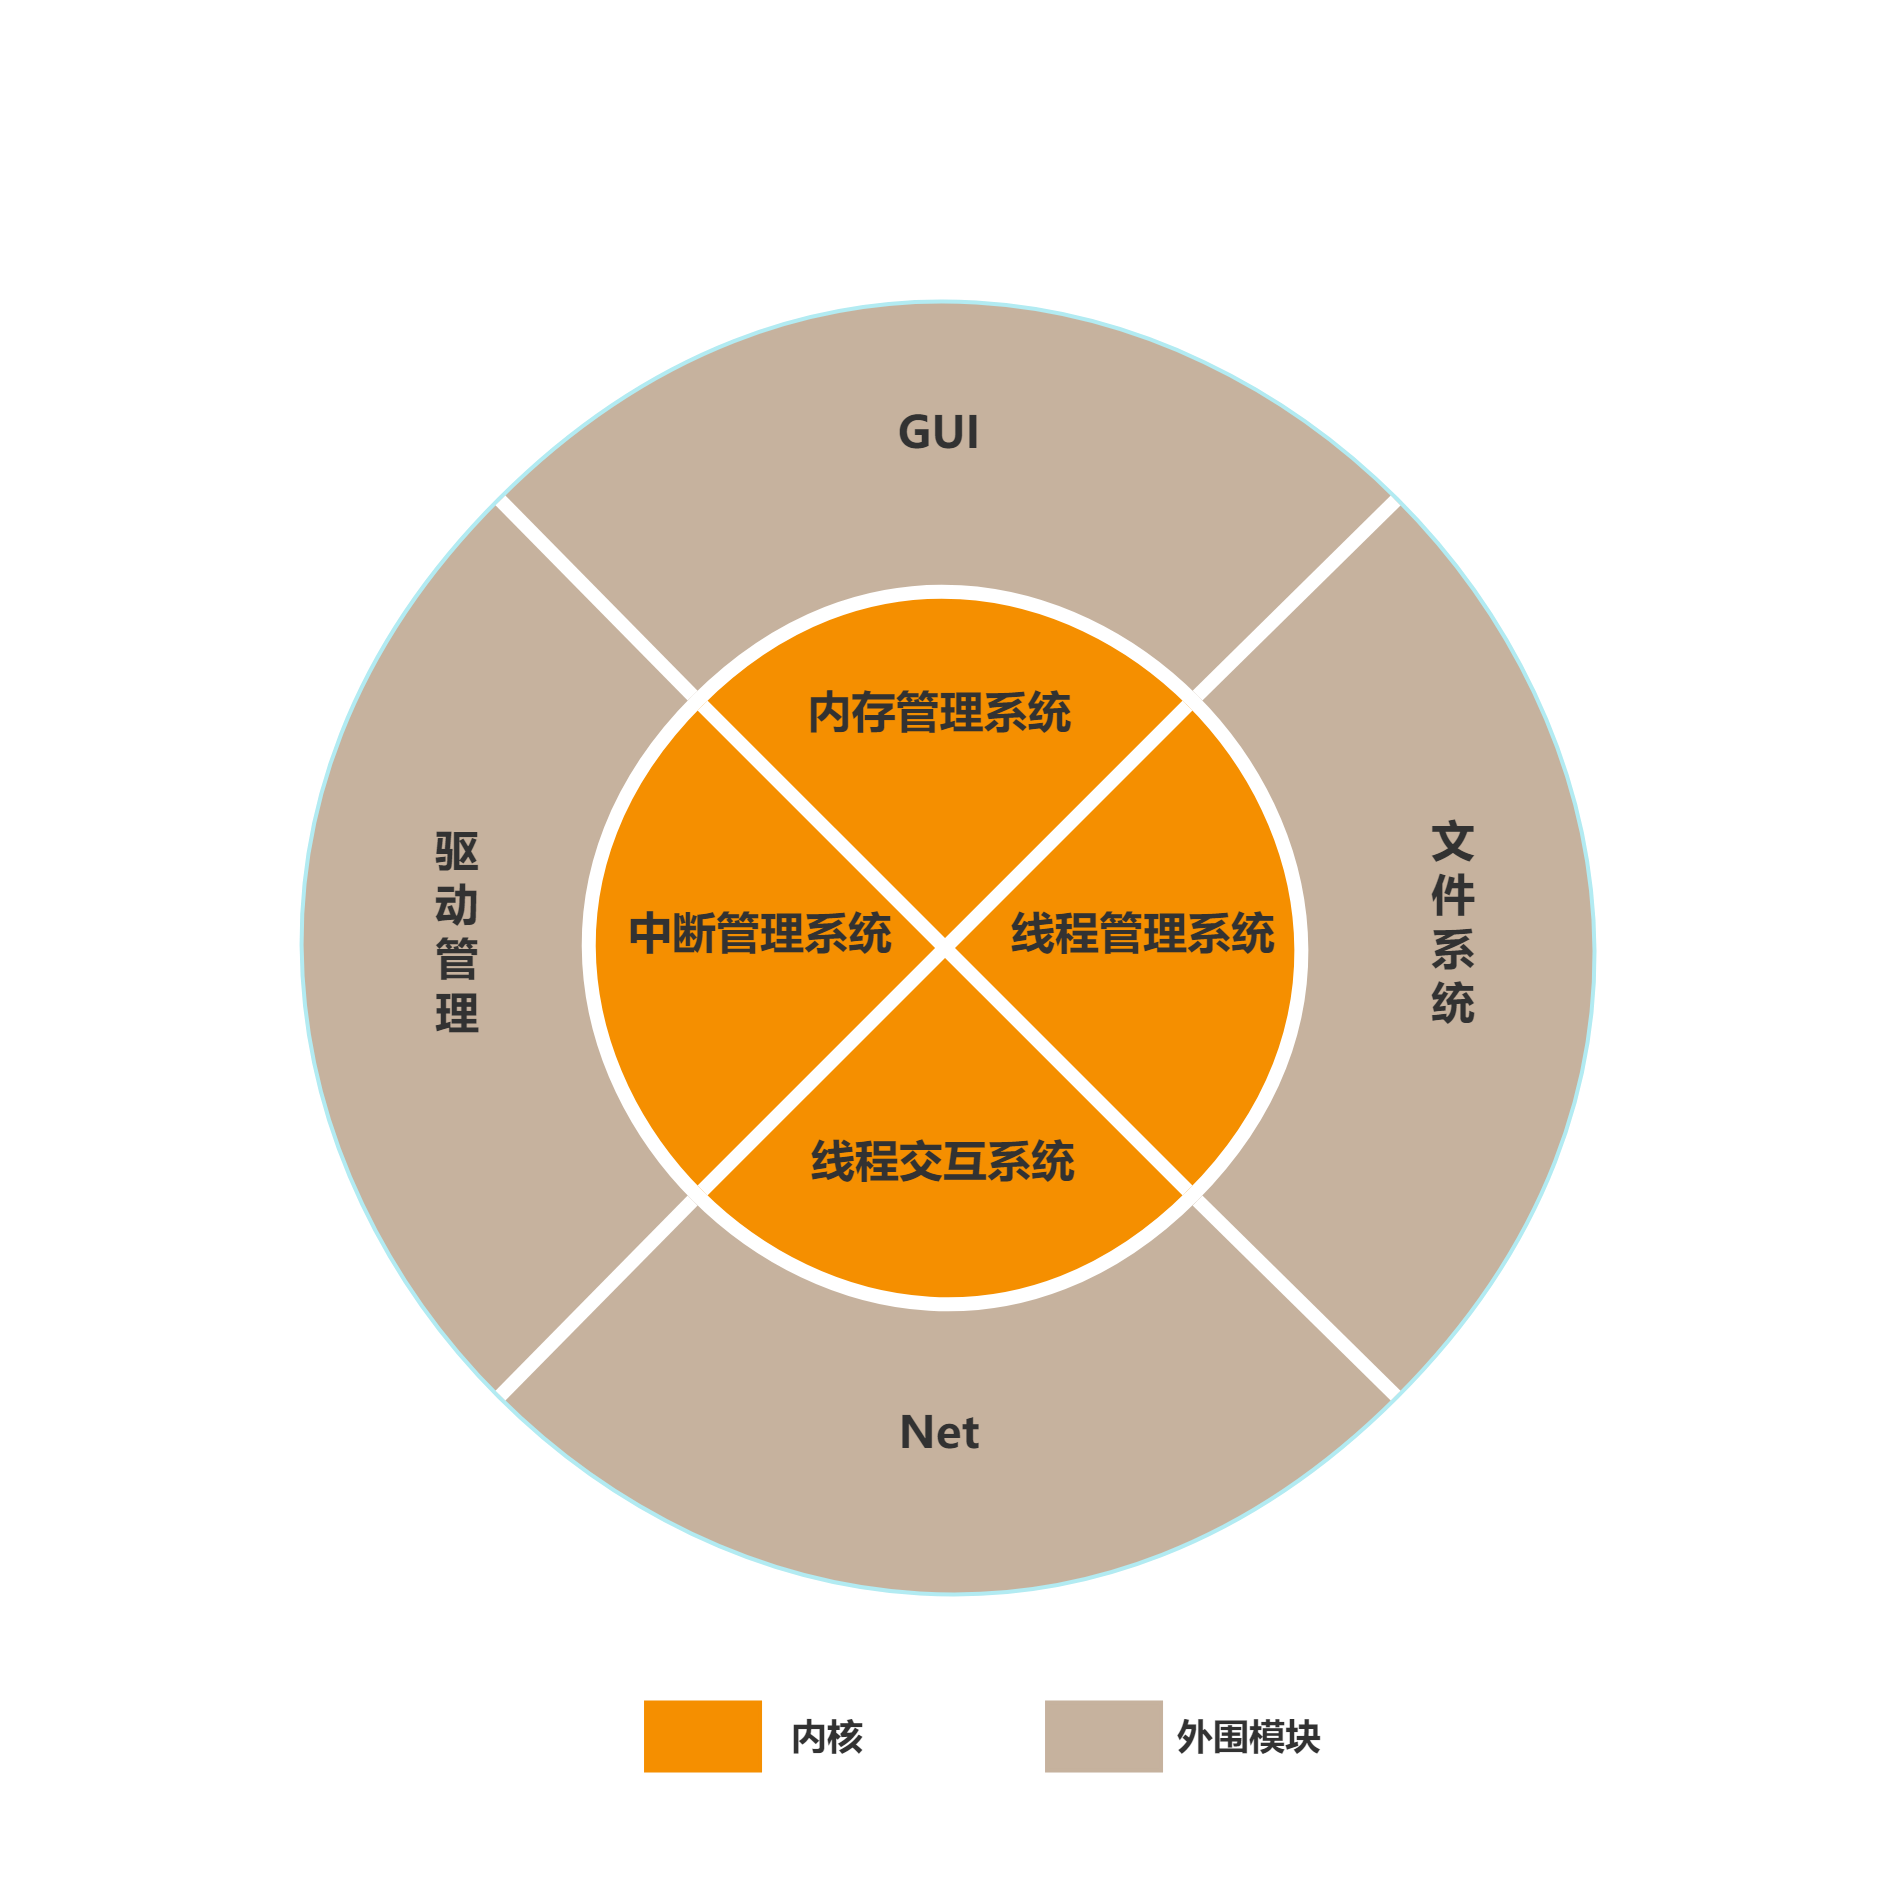
\includegraphics[width=400pt]{aCoral系统结构.png}
	\caption{aCoral系统结构}
	\label{pica}
\end{figure}

内核当中,中断管理系统负责响应并处理处理来自外部和内部的所有中断(异常),例如时钟中断、按键中断等;
内存管理系统负责对mini2440上的SDRAM内存进行管理,包括内存的分配、回收算法的实现;
线程管理系统包括线程调度机制和线程调度策略两个部分,负责创建、挂起、杀死线程等操作以及按照何种策略来调度线程;
线程交互系统包括互斥量、信号量、邮箱、消息队列等线程间交互机制。

\section{aCoral文件结构}

aCoral 的一大特点是可配置性,这就要求好的系统文件结构。aCoral内核主要由7个文件夹组成:

(1)kernel,内核文件夹.该文件夹下又有两个文件夹:

	\chinesespace i. include:内核模块的头文件目录

	\chinesespace ii. src:内核模块的源码目录
 
(2)hal(Hardware Abstract Layer),硬件抽象层文件夹。这里存放各种开发板硬件相关的底层代码。

(3)include,aCoral一些重要配置头文件。

(4)driver,驱动文件夹。此文件夹存放系统的驱动程序:

	\chinesespace i. src,这里存放平台无关驱动模型实现,比如驱动模型,sd 卡驱动模型。

	\chinesespace ii. include, 这里存放平台无关驱动模型的头文件,比如 screen 设备的信息结构,触摸屏设备的信息结构。

	\chinesespace iii. 开发板相关驱动文件夹,s3c2440,s3c2410,每个文件夹下又各自包含include,src 文件夹。

(5)plugin,项目扩展插件目录,比如文件系统,图形系统,TCP/IP 协议栈等等。

	\chinesespace i. src,扩展插件的公共源码。

	\chinesespace ii. include ,扩展插件的公共头文件。

	\chinesespace iii. 具体的扩展插件文件夹。

(6)lib,库目录。

	\chinesespace i. src,源码目录。

	\chinesespace ii. include,头文件

(7)user,用户程序目录。

	\chinesespace i. src,源码目录。user.c 中的 user\_main 是用户程序的入口函数,大家可以在这个函数里添加自己的应用。

	\chinesespace ii. include,头文件

(8)test,测试文件目录。主用用于内部测试。

	\chinesespace i. src,源码目录。

	\chinesespace ii. include,头文件

除了这些文件夹以外,aCoral根目录下还有一些重要的文件,Makefile、.config(menuconfig自动生成)……
这些文件都有十分重要的作用,可以有空自行学习。另外那些acoral打头的文件则是在编译过程中自动生成的一些辅助文件,有助于开发人员debug和开发应用。
